\section{Backend}


\begin{frame}{Backend}
	\begin{itemize}
		\item Python Server mit Flask API
		\begin{itemize}
			\item stellt Endpunkte zum Persistieren der Stammdaten
			\item stellt Endpunkte zur Live Administration einer Übung
			\item stellt Endpunkte zur Teilnahme an einer Übung
		\end{itemize}
	\end{itemize}
\end{frame}


\begin{frame}{Backend-Komponenten}
	\centering
	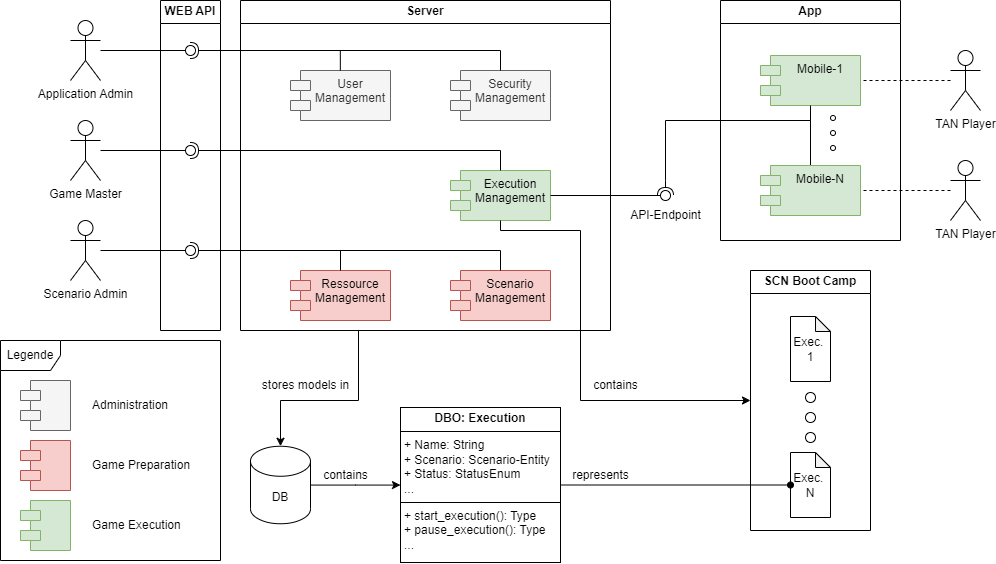
\includegraphics[width=0.7\textwidth]{images/server/component_diagram.png}
\end{frame}


\begin{frame}{Laufzeitobjekte}
	\centering
	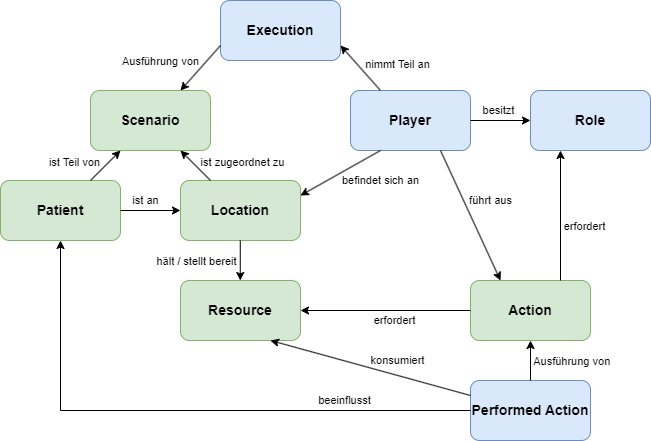
\includegraphics[height=.86\textheight]{images/server_laufzeit_objekte.png}
\end{frame}


\begin{frame}{Datenbankobjekte}
	\centering
	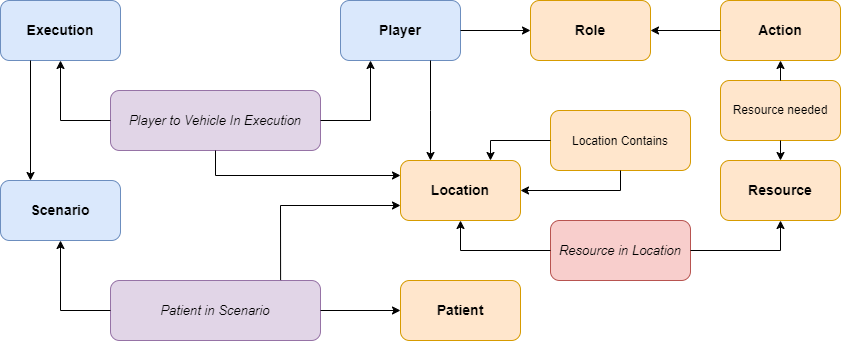
\includegraphics[width=\textwidth]{images/server_datenbank_objekte.png}
\end{frame}
